\subsection{Representations of Lie Groups and Algebras}
In quantum mechanics, the state space $V$ is often a L2 space (like $L^2(\bR^3)$) or some subspace thereof. For a variety of reasons, we are interested in the linear operators on the state space $V$.

\subsubsection{}
We first assume $V$ is finite-dimensional. A finite-dimensional (ordinary) representation of a Lie group $G$ is a homomorphism $G \rightarrow GL(V)$, the set of invertible linear maps on $V$. Similarly, a finite-dimensional (ordinary) representation of a Lie algebra $\mathfrak g$ is a homomorphism $\mathfrak g \rightarrow gl(V)$, the set of linear maps on $V$.

\subsubsection{}
In quantum mechanics, $V$ is also a Hilbert space, so we are often interested in unitary operators: operators that preserve the inner product. Call a representation $\Pi$ of $G$ a unitary representation if $\Pi(G) \subset U(V)$.

Recall that two vectors in the state space that differ by multiplication by a constant are considered to represent the same physical state. Thus we are also interested in the projective unitary group, i.e.
\[
    \frac{U(V)}{\{e^{i\theta}I\}} = PU(V).
\]
A finite-dimensional projective unitary representation is a homomorphism $G \rightarrow PU(V)$. Note that projective unitary representations are different from ordinary representations, so we have to handle them slightly differently.

Nevertheless, the spaces $U(V), PU(V)$ are both Lie groups. Denote their corresponding Lie algebras as $u(v)$ and $pu(v)$.

\subsubsection{}
Suppose we have a (ordinary) representation $\Pi: G \rightarrow GL(V)$. Note if $W$ is an invariant subspace of $V$ under $\Pi(G)$, then we obtain a natural representation $\Pi': G \rightarrow GL(W)$.

Call a (ordinary) representation $\Pi$ irreducible if we cannot create new non-trivial representations in this way. In other words, $\Pi$ is irreducible if the only invariant subspaces of $V$ under $\Pi(G)$ are 0 and $V$.

We achieve a similar definition of an irreducible projective unitary representation $\Pi: G \rightarrow PU(V)$ by considering invariant subspaces of $V$ under all $U$ such that $[U] \in \Pi(G)$.

Colloquially, if $\Pi$ is given, we sometimes say that $W$ ``is a representation of $\Pi$" if $W$ is a invariant subspace.

\subsubsection{}
Given an ordinary representation $\Sigma: G \rightarrow U(V)$, we can get a projective unitary representation $\Pi: G \rightarrow PU(V)$ by composing with the natural map $Q: U(V) \rightarrow PU(V)$. We can ask the converse: can we de-projectivize each $\Pi: G \rightarrow PU(V)$ into a map $\Sigma: G \rightarrow U(V)$? This is generally not possible. However, we can de-projectivize at the Lie algebra level:
\begin{figure}[H]
    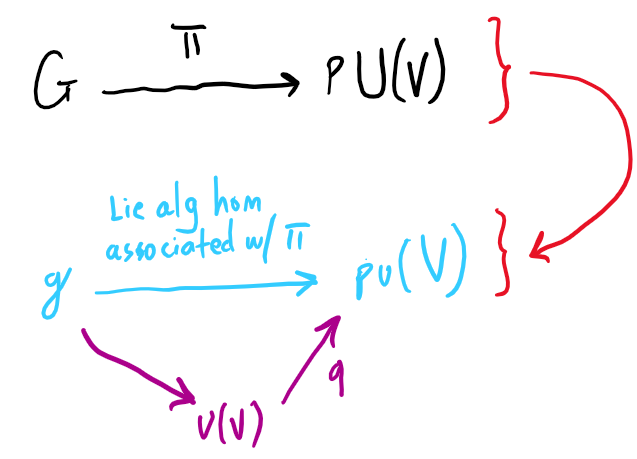
\includegraphics[width=0.5\textwidth]{figures/de-projectivization}
    \centering
\end{figure}

Here, $q: u(v) \rightarrow pu(v)$ is the Lie algebra homormorphism associated with $Q$.

\subsubsection{}
We can also de-projectivize at the expense of passing from $G$ to the universal cover $G^*$.
\begin{figure}[H]
    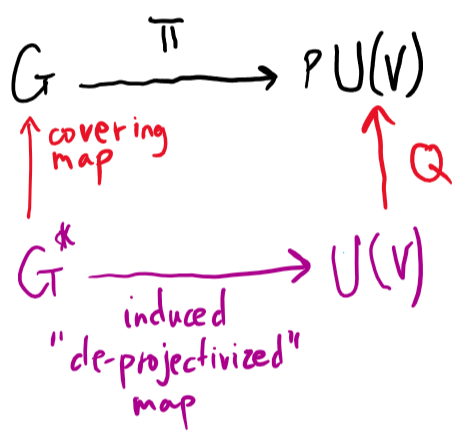
\includegraphics[width=0.4\textwidth]{figures/de-projectivization2}
    \centering
\end{figure}

\subsubsection{}
So far, we have only been considering finite-dimensional representations. In the case that $V$ is infinite-dimensional, we have analogous definitions of ordinary representations and projective unitary representations, albeit with a few extra conditions (like strong continuity).
